\section{Documentation of performance after optimization}
Lets check if our optimizations are indeed correct based on our research and current results.\\
We start out by once again, running the program program with a profiler.

\begin{figure}[h]
    \caption{Profiler Flame Chart}
    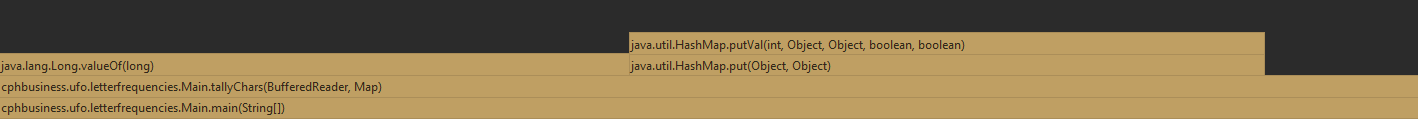
\includegraphics[width=\linewidth]{figures/java_profiler_changed_1.png}
    \label{fig:call-tree-unchanged}
\end{figure}

\begin{figure}[h]
    \caption{Profiler Flame Chart}
    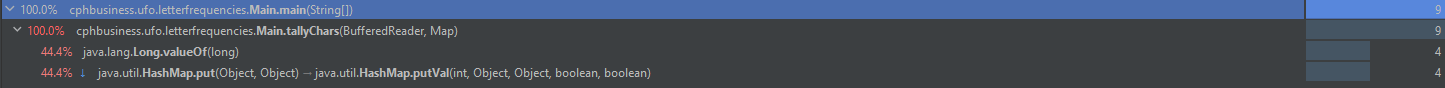
\includegraphics[width=\linewidth]{figures/java_profiler_changed_2.png}
    \label{fig:call-tree-unchanged}
\end{figure}

Just by looking at the profiler, it seems promising that our program will indeed be running less expensive.
To backup the profiler, we perform the same calculations as we did before the optimizations:

\begin{lstlisting}[]
        
        Optimized data

Count:                  10
Sum:                    461.7976
Mean:                   46.17976
Variance:               201.1248140124
Standard Deviation:     14.181848046443 
\end{lstlisting}

\vspace{30px}
Now lets compare it to our earlier results.
\vspace{20px}

\begin{lstlisting}[]        
        Unoptimized data

Count:                  10
Sum:                    820.2117
Mean:                   82.02117
Variance:               866.8134585601
Standard Deviation:     29.441695918546
\end{lstlisting}

\newpage

As we can see from our data, small changes to the code can result in HUGE improvements to the execution times, which further reinforces our statement, that it is important to research the methods you're going to use before writing the program.\\\\

Our data confirms that we reached an average performance gain of 56.30\%, which is greater than our goal of reaching at least 50\% optimization.